\chapter{Quantifying Uncertainties in RANS CFD Simulations}

The Navier-Stokes equations are a set of non-linear partial differential equations that describe the motion and behavior of fluids. Broadly, there are two classes of forces acting on a fluid, inertial and viscous. (TODO Citation) Inertial forces refer to those exerted by the fluids momentum, or its lack thereof. Imagine the force exerted by water coming out of a tap, versus that which is exerted by water coming out of a fire hose. The second situation exerts significantly higher inertial forces. Viscous forces are a result of the fluid's resistance to deformation. Viscosity is a measure of this resistance. It is a property specific to the fluid in question. Honey is more viscous than water. The effect of these viscous forces can be seen if both fluids are poured out of a container. Honey is more resistant to this deformation, and flows out more slowly than water.

The ratio of the inertial and viscous forces on a fluid determines the fluid's behavior in motion. Reynolds number $\left ( Re = \frac{\rho u L}{\mu}\right )$ is a measure of this ratio. When the inertial forces acting upon a fluid are small when compared to the viscous forces, i.e. the Reynolds number is low, the fluid flow is described as \textit{laminar}. This flow is characterized as smooth, without significant cross-currents or time dependence. Laminar flow usually occurs at lower fluid velocity, is relatively easy to predict computationally, and doesn't require any simplifying models.(TODO Citation) 

Fluid flow turns \textit{turbulent} when the ratio of inertial to viscous forces is high, i.e. at high Reynolds numbers. Turbulence refers to the chaotic, time-dependent, varied-scale fluctuations in flow variables that characterize turbulent flows. It's unsteady nature, and the range of length and time scales of the flow eddies, make it computationally intractable to predict exactly. Simplifying assumptions are required to make the computations feasible and productive in an engineering situation. 

Note the ambiguous use of "low" and "high" to describe the Reynolds numbers for laminar and turbulent flow. This is intentional. The point of transition between the two regimes is highly dependent on the fluid and the geometry of the flow itself. This is an active area of research (TODO Citation). This thesis is focused on turbulent flows. 

\section{Turbulent Flows}

In the realm of engineering, there is often a need to predict the behavior of fluid flow in and around engineered products. These situations can range from simulating the flow around an airplane, to simulating the flow through the cooling system in a laptop. Computational Fluid Dynamics (CFD) is the field of study that involves the use of computers and complex numerical analysis techniques to solve the non-linear Navier-Stokes equations on the flow domain of interest. (TODO Citation) As computational capabilities have increased over the past few decades, so has the reliance on the predictive capability of CFD simulations. 

This is made more difficult due to turbulence. The range of length, and time scales that need to be resolved through spatial, and temporal discretization make it computationally intractable to solve exactly (without any simplifying models). Most flows of engineering interest are plagued by turbulence. The difficulty in solving these flows exactly has paved the way for the development of a hierarchy of solution techniques that trade computational cost for prediction accuracy. 

\begin{figure}
    \center
    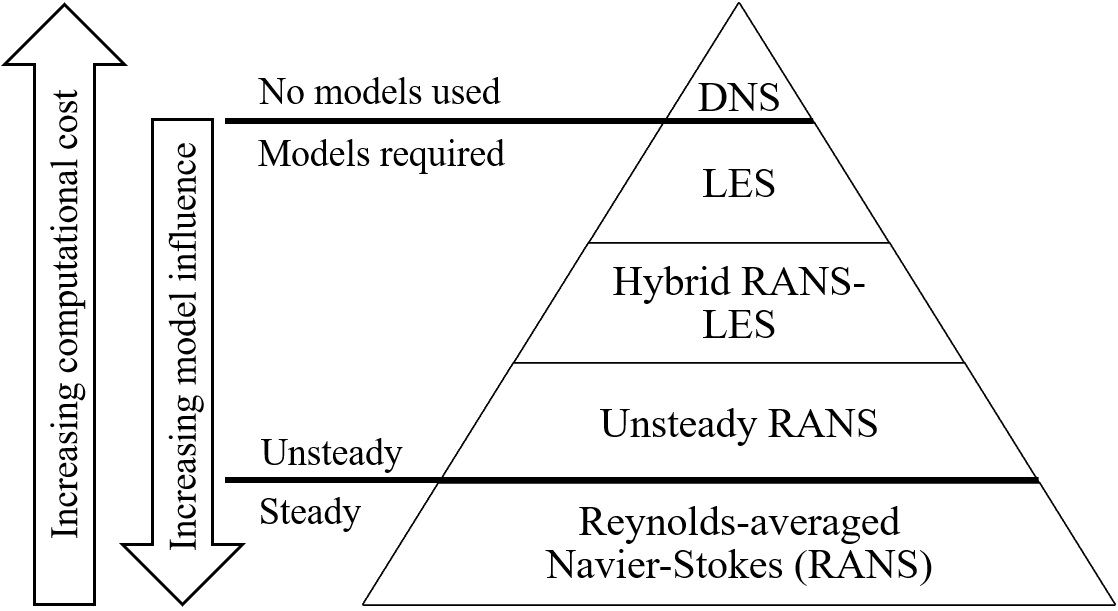
\includegraphics[width=0.75\textwidth]{suthesis/images/solution_heirarchy_simple.png}
    \caption{Heirarchy of CFD solution techniques in order of increasing computational cost and decreasing model influence. \label{fig:cfd_types}}
\end{figure}

Figure \ref{fig:cfd_types} presents this hierarchy in the form of a pyramid. Sitting at the top of this pyramid are Direct Numerical Simulations, or DNS. These calculations do not employ any mathematical models and resolve all spatial and temporal time scales to give an exact reproduction of the fluid behavior. These time-varying (unsteady) simulations are computationally expensive and memory intensive. At the time of writing, DNS calculations are only possible at low Reynolds numbers and for simple geometries such as flat plates \cite{hoyas_reynolds_2008}, and channels \cite{laval_marquillie_dns_channel,marquillie_instability_2011}. This disqualifies the use of DNS, in its current state, for practical engineering applications. 

Below DNS, in Figure \ref{fig:cfd_types}, lie Large Eddy Simulations (LES) and Hybrid RANS-LES simulations. These unsteady simulations resolve some, but not all, of the scales of turbulence. Any time and length scales that aren't resolved, are modeled using some simplifying assumptions (TODO Citation). These solution methodologies allow for the fine-tuning of the desired influence of simplifying models through the chosen level of spatial and temporal discretization. They are in the process of being adopted by industry for specific use cases such as performance predictions for high-lift configuration aircrafts (TODO Citation), or engine simulations (TODO Citation). 

At the base of the pyramid is the most widely used method in industry, Reynolds-averaged Navier-Stokes (RANS) simulation. These simulations suffer the most from modeling inaccuracies. They assume that the flow is steady (no time-dependent variation in flow), and require simplifying turbulence models that aggregate the effects of the turbulent eddies that would be present in the flow. This significantly reduces the computational cost but inhibits the flow features that can be captured by the simulations. While it's unsteady counterpart can resolve some of the time variation of the flow, turbulence modeling is still required which affects the prediction accuracy. Steady RANS simulations are very computationally efficient and can be used for expensive undertakings such as iterative aerodynamic shape optimization (TODO Citation), and aircraft database generation (TODO Citation). This chapter will focus on quantifying the uncertainties that are injected by turbulence models that are employed in RANS simulations. 

\section{Uncertainty and Error in RANS Simulations}

In order to use steady RANS simulations to design engineering products, it is essential to understand its strengths and shortcomings. The extensive use of mathematical models to accelerate these simulations makes it feasible to run multiple function evaluations at different test conditions. Concurrently, the inadequacy of the models in predicting real-world behavior of fluids limits its use to flow conditions where the models are valid. These restrictions have been found over the years through thorough verification and validation of CFD codes and turbulence models (TODO Citation). 

To have a productive discussion of uncertainties and errors in these simulations, precise language is required. For this purpose, definitions and guidelines established by the American Institute of Aeronautics and Astronautics (AIAA) in \cite{computational_fluid_dynamics_committee_guide_1998} are followed. In a non-academic setting, \textit{error} and \textit{uncertainty} are often used interchangeably. To avoid ambiguity, uncertainty is defined as: 
\say{A potential deficiency in any phase or activity of the modeling process that is due to lack of knowledge} \cite{computational_fluid_dynamics_committee_guide_1998}. 

This is contrasted with the definition of error: 
\say{A recognizable deficiency in any phase or activity of modeling and simulation that is not due to lack of knowledge} \cite{computational_fluid_dynamics_committee_guide_1998}. Two key differences surface from these definitions: 

\begin{enumerate}
    \item \textbf{Potential vs. recognizable deficiency -} The effects of the uncertainty in some model may or may not cause a knowable deficiency in the resulting prediction. On the other hand, deficiencies introduced due to modeling errors are identifiable upon examination. 
    
    \item \textbf{Lack of knowledge -} Uncertainty is caused due to lack of knowledge of some physical aspect of what is being simulated. Errors exist even with complete knowledge and often have established practices and methods that can be used to reduce them.  
\end{enumerate}

To solidify these definitions with examples, consider the uncertainty introduced by turbulence models in contrast to discretization errors caused by insufficient grid resolution. Turbulence models are used to 

For example, a turbulence model might introduce deficiencies when making predictions for an aircraft in its high-lift configuration (TODO Citation), whereas it might not introduce any deficiency in predicting the flow around the aircraft in it's cruise configuration. Without a comparison with experimental data, the deficiency is not knowable.

\section{Eigenspace Perturbation Methodology}

\section{Validation}

\section{Application to NASA CRM}
